\documentclass[aspectratio=169,10pt]{beamer}
%
% Choose how your presentation looks.
%
% For more themes, color themes and font themes, see:
% http://deic.uab.es/~iblanes/beamer_gallery/index_by_theme.html
%
\mode<presentation>
{
  \usetheme{Boadilla}      % or try Darmstadt, Madrid, Warsaw, ...
  \usecolortheme{seahorse} % or try albatross, beaver, crane, ...
  \usefonttheme{professionalfonts}  % or try serif, structurebold, ...
  \setbeamertemplate{navigation symbols}{}
  \setbeamertemplate{caption}[numbered]
}
\setbeamersize{text margin left=10mm,text margin right=10mm} 

\usepackage[english]{babel}
\usepackage[utf8]{inputenc}
\usepackage[T1]{fontenc}
\usepackage{hhline}

\usepackage{array}
\usepackage{multirow}

\makeatletter
\newcommand{\thickhline}{%
    \noalign {\ifnum 0=`}\fi \hrule height 1pt
    \futurelet \reserved@a \@xhline
}
\newcolumntype{"}{@{\hskip\tabcolsep\vrule width 1pt\hskip\tabcolsep}}
\makeatother

\usepackage{minted}
\RequirePackage{minted}
%\usemintedstyle{autumn}
\setminted{
    linenos,
    breaklines,
    fontsize=\footnotesize,
    tabsize=4,
    xleftmargin=2em
}
\usepackage{etoolbox}

\makeatletter
\AtBeginEnvironment{minted}{\dontdofcolorbox}
\def\dontdofcolorbox{\renewcommand\fcolorbox[4][]{##4}}
\makeatother

\title{Dissecting Ponzi Schemes on Ethereum}
\subtitle{Identification, Analysis, and Impact\cite{bartoletti2020dissecting}}
\author{Liu Yihao}
%\institute{Where You're From}
\date{\today}

\AtBeginSubsection[] % Do nothing for \section*
{
  \begin{frame}<beamer>
    \frametitle{Outline}
    \tableofcontents[sectionstyle=show/shaded,subsectionstyle=show/shaded/shaded]
  \end{frame}
}


\begin{document}

\begin{frame}
  \titlepage
\end{frame}

\section{Introduction}

\begin{frame}<beamer>
    \frametitle{Outline}
    \tableofcontents[sectionstyle=show/shaded,subsectionstyle=show/shaded/shaded]
\end{frame}

\begin{frame}{Ethereum}

\begin{block}{Definition}
Ethereum\cite{wood2014ethereum} is a decentralized open source blockchain featuring \structure{smart contract} functionality.
\end{block}

\begin{figure}
    \centering
    
\includegraphics[width=0.4\textwidth]{images/ethereum.png}
    \caption{The logo of Ethereum.}
    \label{fig:ethereum}
\end{figure}

\end{frame}

\begin{frame}[fragile]{Smart Contracts}

Smart Contracts are often programmed in the language \structure{Solidity}\cite{dannen2017introducing}.

\pause

\begin{minted}{solidity}
contract AWallet {
    address owner;
    mapping (address => uint) public outflow;
    mapping (address => uint) public inflow;

    function AWallet() { owner = msg.sender; }

    function pay(uint amount, address recipient) returns (bool) {
        if (msg.sender != owner || msg.value != 0) throw;
        if (amount > this.balance) return false;
        outflow[recipient] += amount;
        if (!recipient.send(amount)) throw;
        return true;
    }

    function () { inflow[msg.sender] += msg.value; }
}
\end{minted}

\end{frame}

\begin{frame}{Ponzi Scheme}
\begin{block}{Definition \footnotemark}
A Ponzi scheme is an investment fraud that returns money to existing investors from funds contributed by new investors. \medskip
    
Ponzi scheme organizers often attract new investors by promising high returns with little or no risk. \medskip

Ponzi schemes require a constant 
flow of money from new investors to continue. Ponzi schemes inevitably collapse, most often when it becomes difficult to find new investors or when a large number of investors ask for their funds to be returned. 
\end{block}

\footnotetext[1]{\url{www.sec.gov/spotlight/enf-actions-ponzi}}

\end{frame}

\begin{frame}{Smart Ponzi Scheme}

Implementing Ponzi schemes as smart contracts would have several attractive features: \bigskip

\begin{itemize}
\item The initiator of a Ponzi scheme could stay anonymous.
\item Smart contracts are ``unmodifiable" and ``unstoppable", no central
authority can revert its effects in order to refund the victims.
\item Investors may gain a false sense of trustworthiness from the fact that the
code of smart contracts is public and immutable, and their execution is
automatically enforced.
\end{itemize}

\end{frame}


\section{Ponzi Schemes on Ethereum}

\subsection{Identification}

\begin{frame}{Identification of Ponzi Schemes}

Contracts likely to be Ponzi Schemes: \bigskip

\begin{columns}
\begin{column}{0.32\textwidth}
\begin{figure}
    \centering
    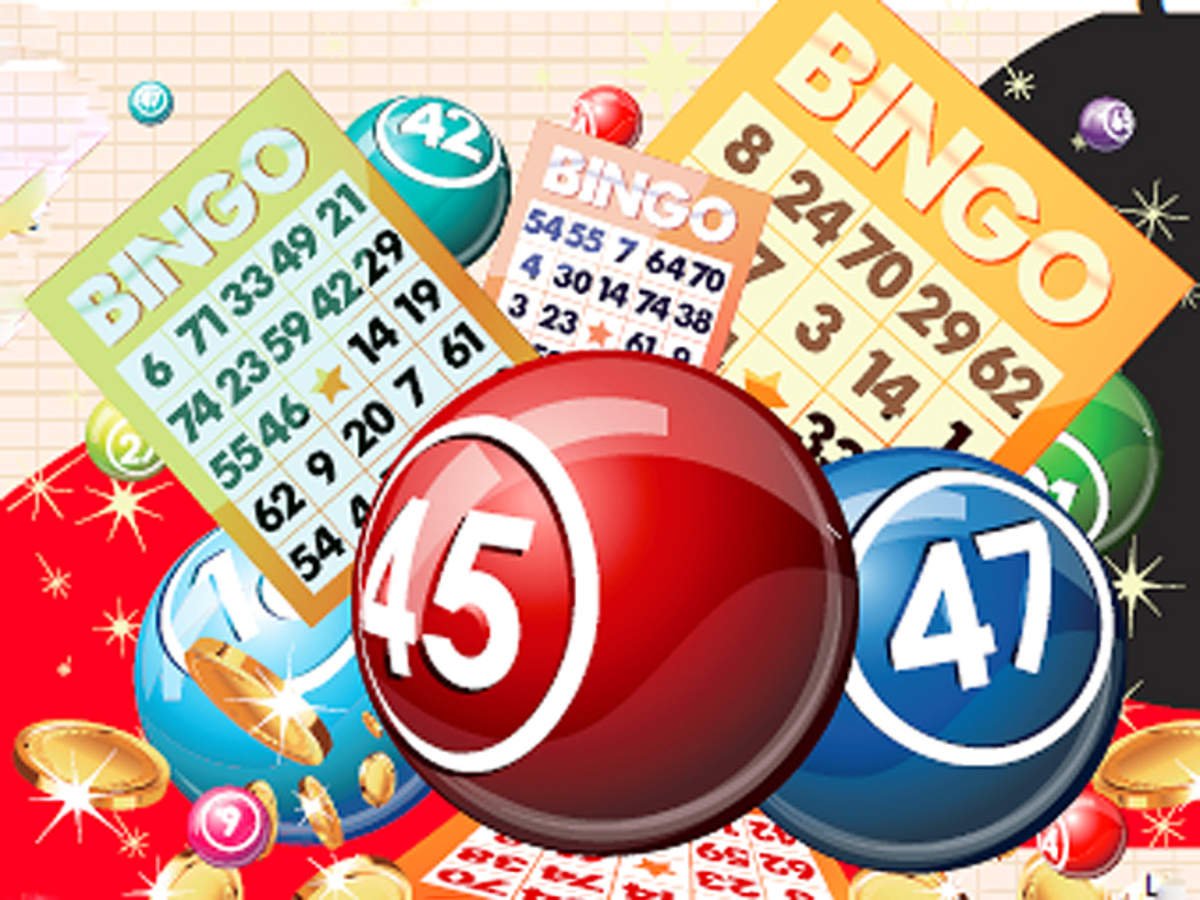
\includegraphics[width=0.9\textwidth]{images/lottery.jpg}
    \caption{Gambling games and lotteries.}
    \label{fig:ponzi-1}
\end{figure}
\end{column}
\begin{column}{0.32\textwidth}
\begin{figure}
    \centering
    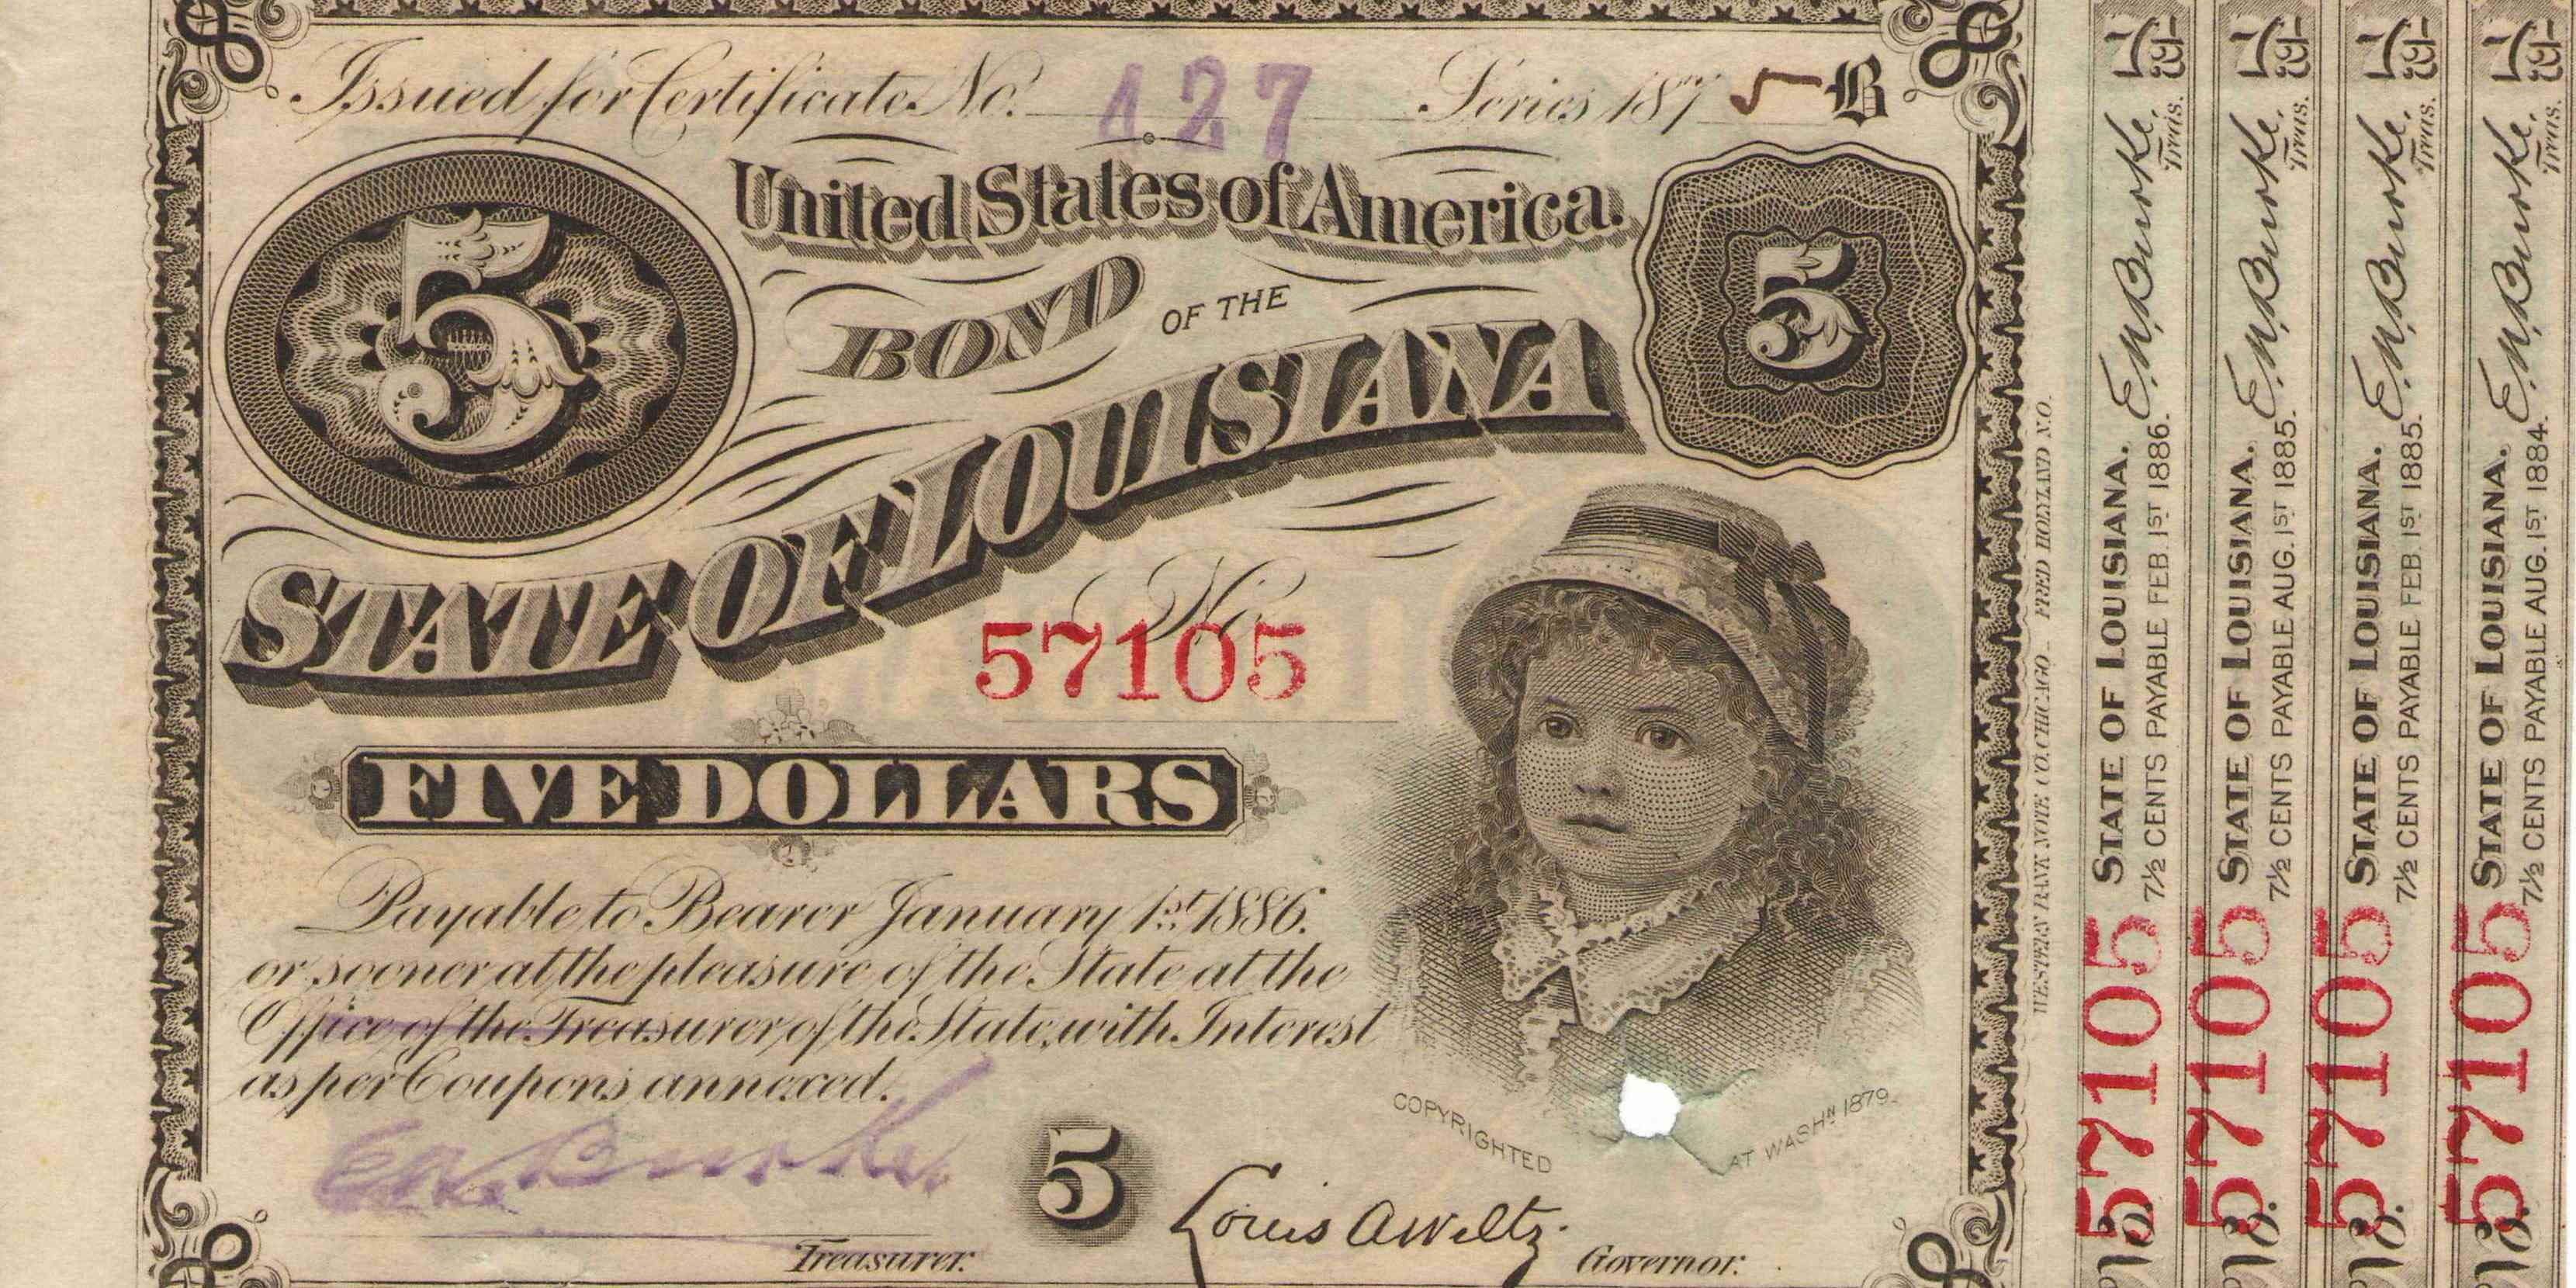
\includegraphics[width=0.9\textwidth]{images/bonds.jpeg}
    \caption{Insurances and bonds.}
    \label{fig:ponzi-2}
\end{figure}
\end{column}
\begin{column}{0.32\textwidth}
\begin{figure}
    \centering
    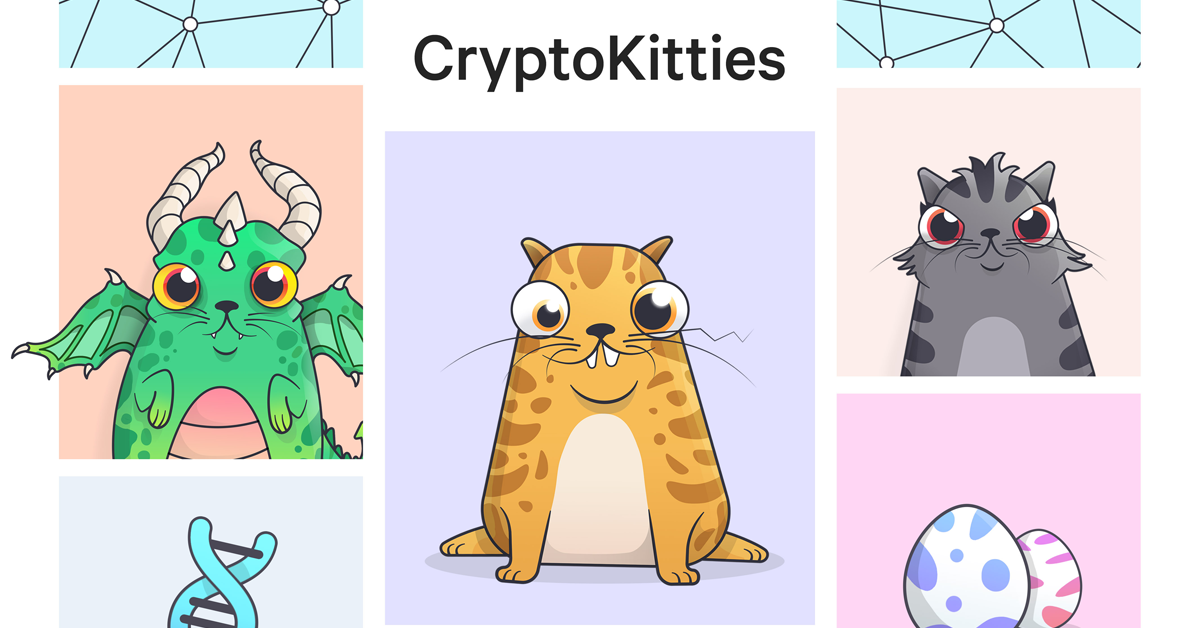
\includegraphics[width=0.9\textwidth]{images/cryptokitties.png}
    \caption{Blockchain games.}
    \label{fig:ponzi-3}
\end{figure}
\end{column}
\end{columns}

\end{frame}


\begin{frame}{Criteria for Classifying a Contract as a Ponzi Scheme}

\only<1-4>{
\begin{block}{Requirement 1}
The contract distributes money to \structure{investors}.
\end{block}
}

\only<1>{\bigskip
\begin{itemize}
    \item Most contracts studied satisfy this requirement
    \item Rules out some contracts such as cryptocurrency exchanges
\end{itemize}
}

\only<2-4>{
\begin{block}{Requirement 2}
The money gathered by the contract comes from investors, \structure{only}.
\end{block}
}

\only<2>{\bigskip
Rules out the cases where the money comes from external sources (eg. a bookmaker)
}

\only<3-4>{
\begin{block}{Requirement 3}
Each investor makes a profit, if \structure{new investors} continue to send money to the contract.
\end{block}
}

\only<3>{\bigskip
Rules out the cases where an unlucky investor
is not guaranteed to make any profit:

\begin{itemize}
    \item Gambling games
    \item Betting
    \item Lotteries
\end{itemize}
}

\only<4-5>{
\begin{block}{Requirement 4}
The \structure{risk of losing} one’s investment grows with the time one
joins the scheme.
\end{block}
}

\only<5>{\bigskip
Many Blockchain games are blamed to be \structure{Ponzi schemes}, but 
actually they only meet the requirements 1, 2, 3, and they can be called \structure{pseudo-Ponzi schemes}:
\begin{itemize}
    \item CryptoKitties
    \item Fomo3D
    \item PoWH3D (Proof of Weak Hands 3D)
\end{itemize}
}

\end{frame}


\subsection{Analysis}

\begin{frame}{Category of Ponzi schemes}

Ponzi schemes can be further classified by anatomy into several categories:

\begin{itemize}
\item Tree-shaped schemes
\item Chain-shaped schemes
\item Waterfall schemes
\item Handover schemes
\end{itemize}

\end{frame}

\begin{frame}{Category of Ponzi schemes}
\framesubtitle{Tree-shaped schemes}

Characteristic:
\begin{itemize}
\item Use a tree data structure to induce an ordering among users.
\item Whenever a user joins the scheme, she must indicate another user as
\structure{inviter}, who becomes her parent node.
\item If no inviter is indicated, the parent will be the root node (the owner)
\item The money of the new user is split among her ancestors with the logic
that the nearest an ancestor is, the greater her share.
\end{itemize} \bigskip

Some examples:
\begin{itemize}
\item Etheramid
\item DynamicPyramid
\end{itemize}

\end{frame}

\begin{frame}{Category of Ponzi schemes}
\framesubtitle{Chain-shaped schemes}

Characteristic:
\begin{itemize}
\item A special case of tree-shaped schemes, where each node of the tree has exactly one child.
\item The ordering induced among users is linear.
\item The scheme starts paying back users when its balance reaches a predefined value, one at a time, in order of arrival.
\item Usually, the contract owner retains a fee from each investment.
\end{itemize} \bigskip

Some examples:
\begin{itemize}
\item Doubler
\item DianaEthereum
\item ZeroPonzi
\end{itemize}

\end{frame}

\begin{frame}{Category of Ponzi schemes}
\framesubtitle{Waterfall schemes}

Characteristic:
\begin{itemize}
\item Similar to chain shaped-schemes for the user ordering
\item Each new investment is poured
along the chain of investors, so that each can take their share.
\item To ensure that all users receive payouts (requirement 3),
the investments of new users must grow proportionally to the number of users.
\item Usually, the contract owner retains a fee from each investment.
\end{itemize} \bigskip

Some examples:
\begin{itemize}
\item TreasureChest
\item PiggyBank2
\end{itemize}

\end{frame}

\begin{frame}{Category of Ponzi schemes}
\framesubtitle{Handover schemes}

Characteristic:
\begin{itemize}
\item An instance of chain-shaped scheme.
\item The entry toll is increased each time a new investor joins the scheme.
\item The toll of a new investor is given in full to the previous one, the previous investor makes an instant profit.
\item Usually, the contract owner retains a fee from each investment.
\end{itemize} \bigskip

Some examples:
\begin{itemize}
\item KingOfTheEtherThrone
\end{itemize}

\end{frame}

\subsection{Impact}

\begin{frame}{General Statistics of the Ponzi Schemes}

\begin{table}
\begin{tabular}{l|cc|cc|cc}
\thickhline
\multirow{2}{*}{Contract name} & \multicolumn{2}{c|}{Transactions} & \multicolumn{2}{c|}{ETH}  & \multicolumn{2}{c}{Users} \\
 & in & out & in & out & paying & paid \\\hline
\texttt{DynamicPyramid}     & 444 & 143  & 7474 & 7437 & 175 & 51  \\
\texttt{DianaEthereum-x1.8} & 288 & 168  & 5307 & 5303 & 129 & 84  \\
\texttt{Doubler2}           & 395 & 161  & 4858 & 4825 & 211 & 68  \\
\texttt{ZeroPonzi}          & 627 & 499  & 4490 & 4489 & 47  & 28  \\
\texttt{Doubler}            & 156 & 57   & 3073 & 3073 & 92  & 17  \\
\texttt{Government}         & 723 & 846  & 2939 & 2939 & 40  & 27  \\
\texttt{Rubixi}             & 686 & 66   & 1367 & 1363 & 104 & 28  \\
\texttt{ProtectTheCastle2}  & 890 & 1257 & 1332 & 1332 & 101 & 68  \\
\texttt{EthereumPyramid}    & 978 & 339  & 986  & 917  & 327 & 125 \\\hline
Total (184 schemes) & 18925 & 9100 & 43881 & 43332 & 2378 & 1232   \\\thickhline
\end{tabular}
\caption{Top-10 Ponzi schemes by amount of invested ether.}
\end{table}

\end{frame}

\begin{frame}{Statistics by Category of Ponzi Schemes}

\begin{table}
\begin{tabular}{l|c|cc|ccc}
\thickhline
\multirow{2}{*}{Category} & \multirow{2}{*}{Number} & \multicolumn{2}{c|}{ETH}  & \multicolumn{3}{c}{Users} \\
 & & in & out & paying & paid & \% \\\hline
Tree-shaped  & 4   & 410   & 400   & 161  & 83  & 51\% \\
Chain-shaped & 151 & 41514 & 40170 & 1967 & 968 & 48\% \\
Waterfall    & 4   & 452   & 444   & 111  & 82  & 73\% \\
Handover     & 4   & 486   & 483   & 97   & 63  & 64\% \\
Other        & 21  & 1017  & 933   & 42   & 36  & 85\% \\\hline
Total        & 21  & 43881 & 43332 & 2378 & 1232 & 51\%\\\thickhline
\end{tabular}
\caption{Statistics by category of scheme.}
\end{table}

\end{frame}

\begin{frame}{Lifetime of Ponzi Schemes}

\begin{figure}
    \centering
    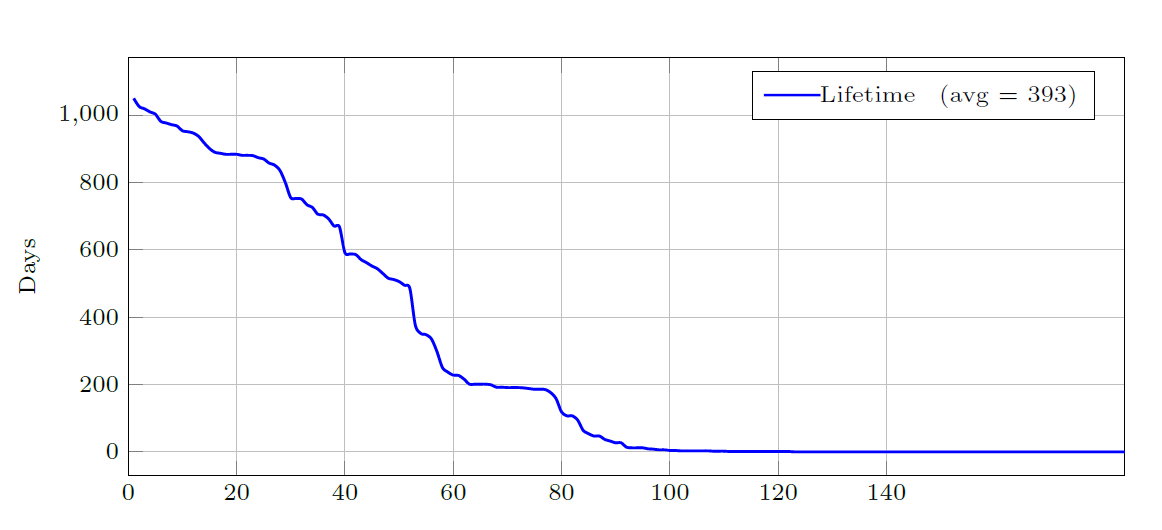
\includegraphics[width=\textwidth]{images/lifetime.png}
    \caption{Lifetime of Ponzi schemes}
    \label{fig:lifetime}
\end{figure}

\end{frame}

\section{Conclusion}

\begin{frame}<beamer>
    \frametitle{Outline}
    \tableofcontents[sectionstyle=show/shaded,subsectionstyle=show/shaded/shaded]
\end{frame}

\begin{frame}{Detect Ponzi Schemes}
\begin{itemize}
\item Check the advertisements
\item Analyze the contract code
\item Analyze the transaction logs
\end{itemize}
\end{frame}

\begin{frame}{Critical Thinking of Methodology Used}

Similarities with other works in analyzing the Bitcoin network:
\begin{itemize}
\item Data Collection and Management
\item Analyze based on categories
\item Analyze based on evolution (time)
\item Measure of the gains and losses of the users
\end{itemize}\bigskip

\pause

Differences:

\begin{itemize}
\item Focus on source code of contrasts
\item Measure of the economic impact of Ponzi schemes
\item Measure of inequality of payments to and from the schemes
\end{itemize}

\end{frame}

\section*{}

\begin{frame}{References}
\bibliographystyle{IEEEtran}
\bibliography{main.bib}
\end{frame}

\begin{frame}
\begin{center}
\Huge
Thank you!
\end{center}
\end{frame}

\end{document}
